\chapter{Теплогидравлический расчет}
\section{Определение термического КПД паротурбинного цикла}

Расчет термического КПД реактора КЛТ-40С проводилось для паротурбинной
установки ТК-35/38-3,4. Основные параметра данной ПТУ приведены в
табл.1.3. Тепловая схема АППУ для данного реактора приведена на рис.2.1.

\begin{figure}[!h]
\center
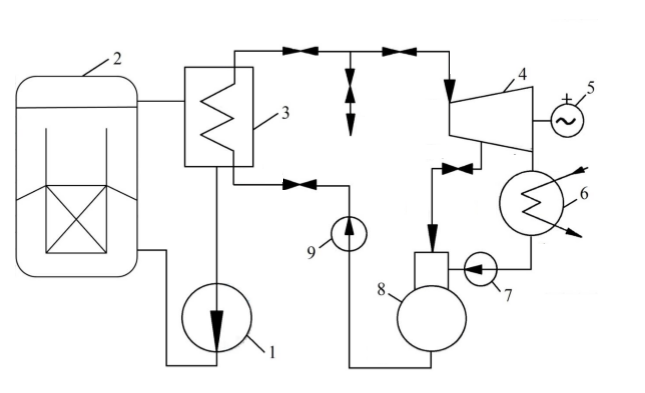
\includegraphics[width=6.49583in,height=3.95764in]{media/image4.png}
\caption{Расчетная тепловая схема АППУ с реактором КЛТ-40С: 1 -
главный циркуляционный насос 1-го контура, 2 -- активная зона ядерного
реактора, 3 -- парогенератор, 4 - ЦВД турбины, 5 -- электрогенератор, 6
-- конденсатор, 7 -конденсатный насос, 8 - диаэратор, 9 -- питательный
насос}
\end{figure}

Данной тепловой схеме соответствует T-S диаграмма, приведенная на рис.
2.2.

\begin{figure}[!h]
\center
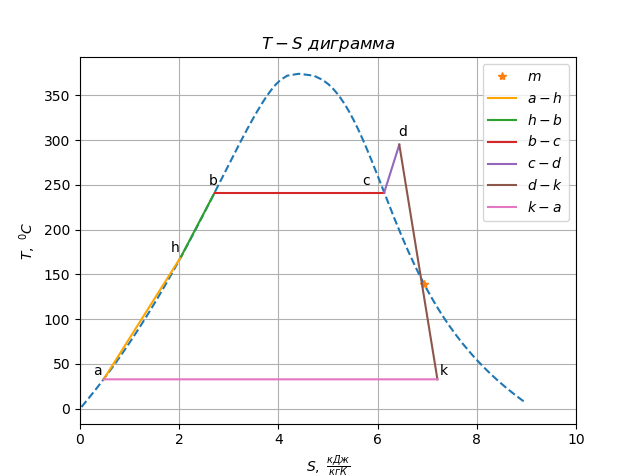
\includegraphics[width=4.56942in,height=3.48958in]{media/image5.png}
\caption{T-S диаграмма : m -- точка регулируемого регенеративного отбора,
a-h -- участок регенеративного отбора, h-b -- экономайзерный участок,
b-c -- испарение, c-d -- пароперегрев, d-k -турбина, k-a - конденсация}
\end{figure}

Для построения данного графика использовались значения из таблицы 2.1,
полученные с помощью программы WaterSteamPro.

Таблица 2.1 - Значения теплофизических параметров на разных участках
тепловой схемы АППУ

Расчет КПД производился по формуле:

\[\eta_{3} = \eta_{0} + \left( \eta_{\infty} - \eta_{0} \right) \cdot \frac{n}{n + 1}\ ,\]

\flushleft где:
\begin{description}
	\item[${n}$] - число регенеративных отборов (в нашем случае \emph{n}=3),
	\item[$\eta_{0}$] - КПД, рассчитываемый без учета регенеративных отборов,
	\item[$\eta_\infty$] - КПД, рассчитываемый при идеальной
	регенерации (т.е. при бесконечном числе отборов).
\end{description}

\[\eta_{0} = 1 - T_{k} \cdot \frac{S_{d} - S_{a}}{i_{d} - i_{a}} = \ 0.3556\]

\[\eta_{\infty} = 1 - T_{k} \cdot \frac{S_{d} - S_{h}}{i_{d} - i_{h}} = 0.4011\]

Тогда получим:

\[\eta_{3} = 0,4149\]

КПД РУ может быть рассчитан по формуле:

\[\eta_{Brutto} = \ \eta_{IT} \cdot \eta_{M} \cdot \eta_{EG} \cdot \eta_{oi} \cdot \eta_{3} = 0.2723\textrm{ ,} \]

где: 
\begin{description}
	\item[$\eta_{IT}$] = 0.98 -- коэффициент использования тепла,
	\item[$\eta_{M}$] = 0.97 -- механический КПД,
	\item[$\eta_{EG}$] = 0.98 -- КПД электрогенератора,
	\item[$\eta_{oi}$] = 0.7 -- внутренний относительный КПД турбины,
	\item[$\eta_{3}$] -- термический КПД, рассчитанный по формуле.
\end{description}

\section{Расчет тепловой мощности и построение T-Q диаграммы}

Зная электрическую мощность (таблица 1.3) и КПД РУ, вычислим тепловую
мощность установки:

\[\ Q =\frac{W}{\eta_{Brutto}} = 128.53\] МВт

Рассчитаем минимальный расход теплоносителя, необходимый для отвода
тепла Q в единицу времени:



\[G_1 = \frac{Q}{{i}_{1}} \cdot 3.6 = 998.7\]кг/с,

где \[{i}_{1}\] -- разность энтальпий 1-го контура (таблица 1.2)

Составим уравнение теплового баланса для 2-го контура:

\begin{equation}
Q = G_2\cdot(i_{ab} + i_{bc} + i_{cd})
\end{equation}

где ${i}_{ab}$ -- разность энтальпий на участке a-b (нагрев
воды 2-го контура до температуры насыщения), ${i}_{bc}$ --
разность энтальпий на участке испарения, ${i}_{cd}$ -- разность
энтальпий на участке пароперегрева (данные взяты из таблицы 2.1)

Тогда для расчета значения G­\textsubscript{2} получаем формулу:

\begin{equation}
G_2 =\frac{Q}{{i}_{ab} + {i}_{bc} + {i}_{cd}} = 57.92
\end{equation}


На основании полученных данных построим T-Q диаграмму (Рисунок 2.2) --
график, показывающий зависимости температур теплоносителя и рабочего
тела от переданного им тепла.

\begin{figure}[!h]
\center
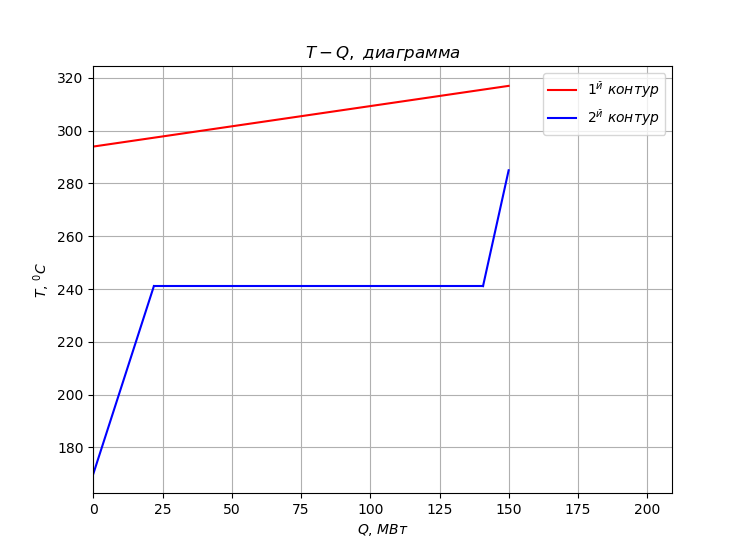
\includegraphics[width=4.56942in,height=3.48958in]{media/image7.png}
\caption{TQ-диаграмма}
\end{figure}

\section{Расчет дополнительных геометрических характеристик ТВС и
активной зоны}

\begin{figure}[!h]
\center
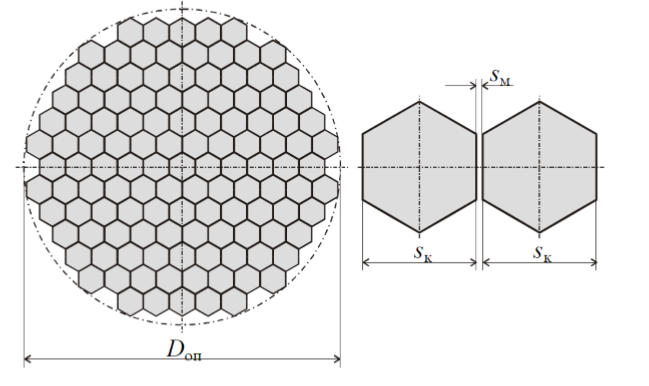
\includegraphics[width=4.56942in,height=3.48958in]{media/image8.png}
\caption{Компоновка ТВС в активной зоне \cite{deev}}
\end{figure}

В таблице 2.2 представлены основные технические характеристики ТВС и АЗ,
которые будут использоваться в дальнейшем.

Таблица 2.2 -- Основные характеристики АЗ

\begin{longtable}[]{@{}|p{10cm}|c|@{}} 
\toprule
Наименование параметра & Значение\tabularnewline
\midrule
\endhead
Тип и форма ТВС & Чехловая с вытеснителем \tabularnewline
Форма вытеснителя & Шестигранная\tabularnewline
Диаметр твэла d\textsubscript{твэл}, мм & 6.8\tabularnewline
Эквивалентный диаметр компенсатора распухания d\textsubscript{комп}, мм
& 2.52\tabularnewline
Шаг решетки твэлов s,мм & 9.6\tabularnewline
Длина активной части твэла H\textsubscript{АЗ}, мм & \centering 1300\tabularnewline
Размер чехла ТВС под ключ s\textsubscript{k}, мм & 96\tabularnewline
Расстояние между ТВС s\textsubscript{м}, мм & 2\tabularnewline
Толщина чехла ТВС $\delta_{tvs},\ mm$ & 1.65\tabularnewline
Количество ТВС, шт & 121\tabularnewline
Количество твэлов N\textsubscript{твэл}, шт & 69\tabularnewline
Количество СВП $\O$ 6.8 мм N\textsubscript{СВП1,} шт & 9\tabularnewline
Количество СВП $\O$ 4.5 мм N\textsubscript{СВП2,} шт & 6\tabularnewline
Толщина оболочки СВП1 $\delta$\textsubscript{СВП1,} мм & 0.5\tabularnewline
Толщина оболочки СВП2 $\delta$\textsubscript{СВП2,} мм & 0.45\tabularnewline
Количество пэлов в кластере вытеснителя, мм & 7\tabularnewline
Толщина оболочки пэла $\delta$\textsubscript{пэл}, мм & 0.5\tabularnewline
Площадь поперечного сечения вытеснителя S\textsubscript{в},
мм\textsuperscript{2} & 689\tabularnewline
Эквивалентный диаметр компенсатора распухания d\textsubscript{комп,} мм
& 2.52\tabularnewline
\bottomrule
\end{longtable}

По данным таблицы 2.2 найдем геометрические параметры АЗ:

описанный диаметр АЗ:

\[D_{op} = \sqrt{\frac{2 \cdot \sqrt{3}}{\pi}N_{TVS}}(S_{k} + S_{m}) = 1132\textrm{ мм}\]

относительный шаг решетки:

\[x = \ \frac{s}{d_{tvel}} = 1.41\]
\begin{center}
эквивалентный диаметр треугольной решетки:

\[d_{ekv} = \ d_{tvel}\left( \frac{2\sqrt{3}}{\pi} \cdot x^{2} - 1 \right)= 8.14 \textrm{ мм}\]


площадь поперечного сечения кассеты:

\[\emph{S­\textsubscript{tvs}} =S­\textsubscript{tvs}\frac{\sqrt{3}}{2} \cdot (s_{k} - 2 \cdot \delta_{tvs}) ^2= 7750.2 \textrm{ мм}^2\]

площадь проходного сечения:


\[\emph{S­\textsubscript{tn }}=S_{tvs} - \ \pi \cdot \left( N_{tvel}\frac{{d_{tvel}}^{2}}{4} + \ N_{svp1}\frac{{d_{svp1}}^{2}}{4} + \ N_{svp2}\frac{{d_{svp2}}^{2}}{4} \right) - S_{v}\]

\[\emph{S­\textsubscript{тн }}= 4133.06 \textrm{мм}\textsuperscript{2}\]

обогреваемый периметр:

\[d_t = N_{tvel} \ \pi \ d_{tvel}=1.474 \textrm{ м}\]
эквивалентный диаметр АЗ:

\[D_{ekv} = \ \sqrt{\frac{2\sqrt{3}}{\pi}\ N_{tvs}}\ \left( s_{k} + s_{m} \right) = 1131.98\ \textrm{мм}\]

объем АЗ:


\[V_{az} = \ \frac{\pi\ H_{az}{D_{ekv}}^{2}}{4} = 1.308\ \textrm{м}\textsuperscript{3}\]
\end{center}

\section{Расчет средних тепловых характеристик активной зоны}

Удельная энергонапряженность АЗ:

\[q_{v} = \ \frac{Q_{t}}{V_{az}} = 98.243\ \frac{MVt}{m^{3}}\]

Средняя тепловая мощность ТВС:

\[Q_{tvs} = \ \frac{K_{Q}Q_{t}}{N_{tvs}}\] = 1.04 МВт , где

\emph{K\textsubscript{Q }}= 0.98 -- коэффициент, учитывающий долю тепла,
выделяющегося в твэлах.

Средний линейный тепловой поток от твэлов:

\[q_{lsr} = \frac{Q_{TVS}}{n_{tvel}H_{a.z}} =\] 11.6 \[\frac{kVt}{m}\]

Средняя плотность теплового потока на поверхности твэлов:

\[q_{sr} = \frac{Q_{TVS}}{F_{to}} = \frac{q_{lsr}}{\pi d_{tvel}} =\]
543.25 \[\frac{kVt}{m^{2}}\]

\section{Расчет распределения температур по высоте для ТВС с
максимальным энерговыделением}

\subsection{Распределение плотности теплового потока по высоте твэла
для ТВСМ}

В первом приближении коэффициенты неравномерности возьмем следующие:

\[k_{r} = 1.42\], \[k_{z} = 1.36\]

Соответственно \emph{k\textsubscript{v}} =
\[k_{r} \cdot k_{z} = 1.9312\]

Исходя из данных коэффициентов неравномерности найдем высоту и радиус
активной зоны с учетом отражателя:

\[k_{z} = \frac{q_{0,z}}{\frac{1}{H}\int_{-H/2}^{H/2}{q_{0,z}\cos{( \frac{\pi z}{H_{ef}} )dz}}} =\frac{H}{H_{ef}}\frac{\pi}{2}\frac{1}{\sin( \frac{\pi H}{2H_{ef}})} = k_{z}\sin( \frac{\pi H}{2H_{ef}}) = \frac{\pi H}{2H_{ef}}\]


\[H_{ef} = 1.55\ m\]

\[k_{r} = \frac{q_{0,z}}{\frac{1}{\pi R^{2}}\int_{0}^{R}{q_{0,r}{\left( \xi_{0}\frac{r}{R_{ef}} \right)dr}}} = \frac{R}{R_{ef}}\frac{\xi_{0}}{2\left( \xi_{0}\frac{R}{R_{ef}} \right)} = > 2k_{r}\left( \xi_{0}\frac{R}{R_{ef}} \right) = \xi_{0}\frac{R}{R_{ef}}\]

\[R_{ef} = 0.9\ m\]

Распределения плотности теплового потока выглядит следующим образом:

\[q\left( z \right) = q_{\max}\cos \pi\frac{z}{H_{eff}} \]

\[q_{l}\left( z \right) = q_{lmax}\cos \pi\frac{z}{H_{eff}} \ ,\]

где \[q_{\max} = \ \emph{k\textsubscript{v} q\textsubscript{ср} =}1.049 \frac{\textrm{МВт}}{\textrm{м}^{2}}\],
\[q_{lmax} = k_{v}q_{lsr} = 11.61\ \frac{\textrm{КВт}}{\textrm{м}} , \emph{z} \in-\textrm{[}\frac{H_{az}}{2};\ \frac{{\ H}_{az}}{2}\textrm{]} \]

\begin{figure}[!h]
\center
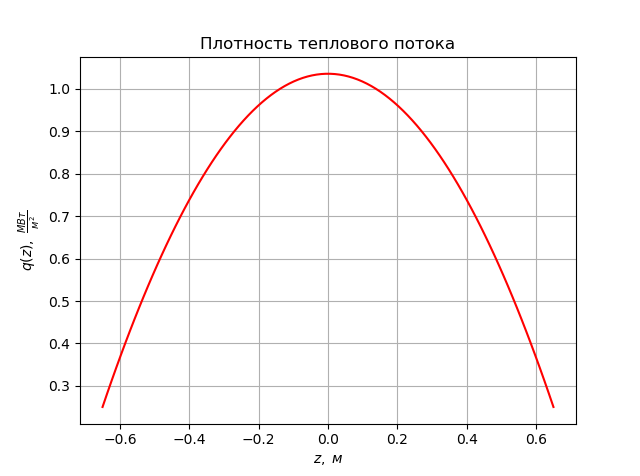
\includegraphics[width=5.11811in,height=3.80659in]{media/image9.png}
\caption{График распределения плотности теплового потока по высоте
твэла для ТВСМ}
\end{figure}

\subsection{Распределение температур во высоте ТВСМ}

Распределение температур теплоносителя по высоте описывается формулой
(2.20):

\[t_{v} = t_{vkh.r} + \frac{k_{G}P_{t}q_{\max}}{k_{Q}G_{tn}S_{p}}\int_{-_{\frac{H_{az}}{2}}}^{z}{cos\left( \pi\frac{z}{H_{eff}} \right)dz}\]

Распределение температуры внешней оболочки твэла:

\[t_{ob.n}\left( z \right) = t_{zh}\left( z \right) + q\left( z \right)R_{\alpha}\],

где \[R_{\alpha} = \ \frac{1}{\alpha}\] .

Для расчета коэффициента теплоотдачи будем использовать следующие
формулы:

\[Nu =  0,0165 + 0,02\left( 1 - \frac{0,91}{x^{2}} \right)x^{0,15} Re^{0,8}\Pr^{0,4}\]

\[w = \ \frac{k_{G}G_{1}k_{r}}{\rho S_{tn}N_{tvs}} = 3.73\ \frac{m}{s}\ ,\]

\[k_{G} = 0,93\] -- коэффициент протечек.

\[Re = \frac{wd}{\nu} = 2.52 \cdot 10^{5}\]

Тогда получим коэффициент теплоотдачи:

\[\alpha\  = \frac{Nu\lambda}{d_{ekv}} = 3.74 \cdot 10^{4}\ \frac{Vt}{m^{2}K}\]

Распределение температуры внутренней оболочки твэла:

\[R_{ob} = \frac{\ln\left( \frac{d_{tvel}}{d_{tvel} - 2\delta_{ob}} \right)}{2\pi\lambda_{ob}},\]

где \[\lambda_{ob} = 18\frac{Vt}{m \cdot K}\] -- теплопроводность
оболочки твэла

\[t_{ob.vn}\left( z \right) = t_{ob.n}\left( z \right) + q_{l}\left( z \right)R_{ob}\]


Распределение температуры топливного сердечника с компенсатором
распухания:

\[t_{ts.t}\left( z \right) = t_{ob.vn}\left( z \right) + q\left( z \right)R_{t.s}\ ,\]

где \[\lambda_{t} = 35\frac{Vt}{m \cdot K}\] -- теплопроводность
ThO\textsubscript{2} в силуминовой матрице в начале кампании,

\[R_{t.s} = \frac{d_{tvel}}{4\lambda_{t} 1 - \left( \frac{d_{komp}}{d_{t.s}} \right)^{2} }\left\{ 1 - \left( \frac{d_{komp}}{d_{t.s}} \right)^{2} 1 - 2\ln\left( \frac{d_{t.s}}{d_{komp}} \right)  \right\}.\]

Все вышеперечисленные зависимости температур представлены на рисунке 2.6

\begin{figure}[!h]
\center
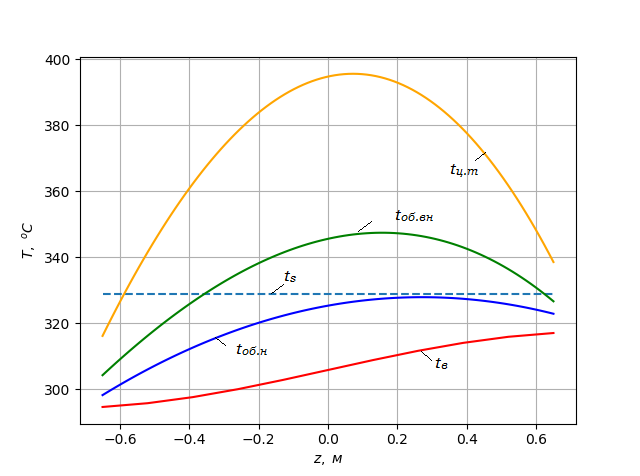
\includegraphics[width=5.11811in,height=3.80712in]{media/image10.png}
\caption{График распределения температур по высоте ТВСМ:
t­\textsubscript{в} - температура теплоносителя, t­\textsubscript{об.н}
-- температура наружной оболочки, t­\textsubscript{об.н} -- температура
внутренней оболочки, t­\textsubscript{т.ц} -- температура топливной в
центре сердечника, t­\textsubscript{s} -- температура насыщения 329.04
$^\circ C$.}
\end{figure}

Таблица 2.3 -- Максимальные температуры В ТВСМ

\begin{longtable}[]{@{}|l|l|@{}} 
\toprule
& t\textsubscript{max,} $^\circ C$.\tabularnewline
\midrule
\endhead
t\textsubscript{об.н} & 328.79\tabularnewline
t\textsubscript{об.вн} & 347.80\tabularnewline
t\textsubscript{ц.т} & 395.98\tabularnewline
\bottomrule
\end{longtable}

\clearpage

\section{Оценка коэффициента запаса до кризиса теплообмена}

Учет отличия теплового диаметра \[d_{t}\] стандартной ячейки от базового
значения:

\begin{equation}
K_{1} = \left( \frac{d_{t}}{9,36} \right)^{- \frac{1}{3}} = 1,112
\end{equation}


Учет относительного шага расположения стержней:

\begin{equation}
K_{2} = 0,2 + 0,57\left( \frac{s}{d} \right) = 1.0037
\end{equation}


Учет влияния на критический тепловой поток входных условий сборки:

\begin{equation}
K_{3} = 1 + 0,6\exp{\left( - \frac{0,01L}{d_{t}} \right) = 1.089}
\end{equation}


Учет турбулизирующего воздействия на кризис кипения дистанционирующих
решеток:

\begin{equation}
K_{4} = 1 + Aexp\left( - \frac{0.01Z}{d_{t}} \right) = 1.2
\end{equation}

\begin{equation}
K = K_{1}K_{2}K_{3}K_{4}K_{5} = 1,136
\end{equation}

\begin{quote}
\[q_{kr} = q_{kr.tab}K\]
\end{quote}


Табличные значения КТП для
\[P = 12,7\ Mpa\ i\ \rho w = 2367\frac{kg}{m \cdot s}\]

Таблица 2.4 -- значения КТП

\begin{longtable}[]{@{}llllllllll@{}}
\toprule
x & -0,4 & -0,3 & -0,2 & -0,1 & 0 & 0,1 & 0,2 & 0,3 & 0,4\tabularnewline
\midrule
\endhead
q\textsubscript{кр.таб}, МВт & 6.48 & 5.60 & 4.46 & 3.29 & 2.47 & 1.85 &
1.29 & 0.81 & 0.47\tabularnewline
q\textsubscript{кр}, МВт & 10.01 & 8.64 & 6.88 & 5.08 & 3.81 & 2.85 &
1.99 & 1.25 & 0.72\tabularnewline
\bottomrule
\end{longtable}

На график (Рисунок 2.7) нанесены значения КТП с учетом поправок, взятые
из таблицы 2.4, а также кривые
\[q_{kr}\left( 1 \pm \sigma_{kv} \right)\], которые характеризуют
возможное расхождение между расчетными значениями и экспериментальными
данными.

\[\sigma_{kv} = 0,15\] -- среднеквадратичное отклонение данных
экспериментов от расчетной формулы или данных таблицы.

\begin{figure}[!h]
\center
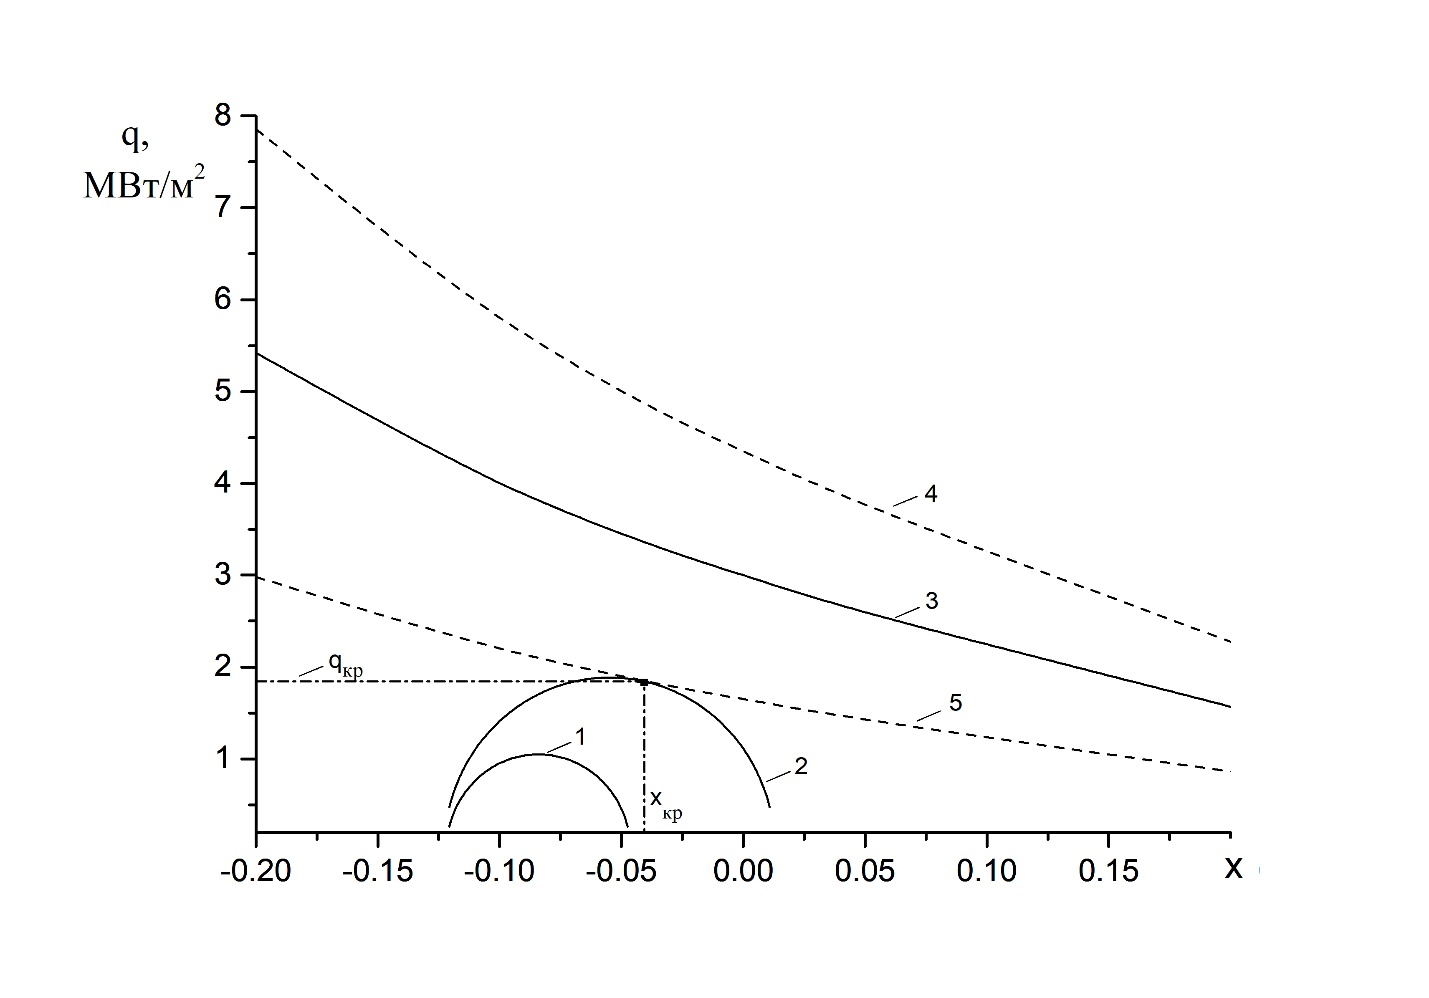
\includegraphics[width=6.49583in,height=4.53750in]{media/image11.png}
\caption{График определения запаса до кризиса теплообмена: 1 --
распределение плотности теплового потока в ТВСМ в номинальном режиме
работы реактора; 2 -- то же, но при увеличении q в 1.8 раза; 3 --
расчетные значения КТП согласно табличному методу; 4,5 -- то же с учетом
возможных отклонений расчетных значений от экспериментальных данных.}
\end{figure}

Из данного рисунка видно, что в точке (\emph{x\textsubscript{кр,}
q\textsubscript{кр}}) кривые 2 и 5 касаются друг друга.

Это означает, что при следующих параметрах \emph{x\textsubscript{кр}} =
-0.04, \emph{q\textsubscript{кр}} = 1.844 существует вероятность
возникновения кризиса теплообмена который может произойти в сечении
ТВСМ, находящемся на расстоянии около 0.8 м от входа в сборку
(\[z_{kr} \approx 1.1\ m\]).

\[K_{zap} = 1.8\]

\section{Расчет гидравлических сопротивлений ТВС}

Полные потери давления при движении теплоносителя в каналах АЗ реактора
вычисляются по следующей формуле:

\[p = p_{tr} + \sum_{}^{}{p_{m} \pm p_{usk} \pm p_{niv}}\]

Коэффициент сопротивления трения:

\[\xi_{0} = {(1,82lgRe - 1,64)}^{- 2} = 0.016\]

\[\frac{\xi}{\xi_{0}} = 1,10 + 0,18\left( x - 1 \right) = 1.17\]

\[\xi = 0.019\]

Перепад давления из-за трения:

\[p_{tr} = \xi\frac{L}{d_{g}}\frac{\rho w^{2}}{2} = 7287\ Pa\]

Таблица 2.5- Коэффициенты местных сопротивлений:

\begin{longtable}[]{@{}llllll@{}}
\toprule
$\zeta$\textsubscript{вх} & $\zeta$\textsubscript{вых} & $\zeta$\textsubscript{н.р} &
$\zeta$\textsubscript{в.р} & 5$\zeta$\textsubscript{др} &
$\Sigma$$\zeta$\textsubscript{м}\tabularnewline
\midrule
\endhead
6 & 4 & 2 & 3 & 0.83 & 15.83\tabularnewline
\bottomrule
\end{longtable}

Падение давления на местных сопротивлениях:

\[p_{m} = \frac{\rho w^{2}}{2}\sum_{}^{}{\xi_{m} = 38.574\ kPa}\]

Потери напора на ускорение:

\[p_{usk} = \left( \rho w \right)^{2}\left( \frac{1}{\rho_{k}} - \frac{1}{\rho_{n}} \right) = 369\ Pa\]

Нивелирный напор:

\[p_{niv} = \left( \rho_{n} - \rho_{k} \right)gH = 339\ Pa\]

Полная потеря давления:

\[p = p_{tr} + p_{m} + p_{usk} - p_{niv} = 54.69\ kPa\]

Затраты мощности на прокачку теплоносителя через активную зону:

\[N = \frac{Vp}{\eta_{n}} = 291.44\ kVt\]

Где V -- объемный расход теплоносителя, \[\eta_{n}\] -- КПД
циркуляционного насоса.

Затраты мощности на прокачку теплоносителя составляет менее 0.83\% от
электрической мощности реактора.
